% Options for packages loaded elsewhere
\PassOptionsToPackage{unicode}{hyperref}
\PassOptionsToPackage{hyphens}{url}
\PassOptionsToPackage{dvipsnames,svgnames,x11names}{xcolor}
%
\documentclass[
  letterpaper,
  DIV=11,
  numbers=noendperiod]{scrartcl}

\usepackage{amsmath,amssymb}
\usepackage{iftex}
\ifPDFTeX
  \usepackage[T1]{fontenc}
  \usepackage[utf8]{inputenc}
  \usepackage{textcomp} % provide euro and other symbols
\else % if luatex or xetex
  \usepackage{unicode-math}
  \defaultfontfeatures{Scale=MatchLowercase}
  \defaultfontfeatures[\rmfamily]{Ligatures=TeX,Scale=1}
\fi
\usepackage{lmodern}
\ifPDFTeX\else  
    % xetex/luatex font selection
\fi
% Use upquote if available, for straight quotes in verbatim environments
\IfFileExists{upquote.sty}{\usepackage{upquote}}{}
\IfFileExists{microtype.sty}{% use microtype if available
  \usepackage[]{microtype}
  \UseMicrotypeSet[protrusion]{basicmath} % disable protrusion for tt fonts
}{}
\makeatletter
\@ifundefined{KOMAClassName}{% if non-KOMA class
  \IfFileExists{parskip.sty}{%
    \usepackage{parskip}
  }{% else
    \setlength{\parindent}{0pt}
    \setlength{\parskip}{6pt plus 2pt minus 1pt}}
}{% if KOMA class
  \KOMAoptions{parskip=half}}
\makeatother
\usepackage{xcolor}
\setlength{\emergencystretch}{3em} % prevent overfull lines
\setcounter{secnumdepth}{5}
% Make \paragraph and \subparagraph free-standing
\ifx\paragraph\undefined\else
  \let\oldparagraph\paragraph
  \renewcommand{\paragraph}[1]{\oldparagraph{#1}\mbox{}}
\fi
\ifx\subparagraph\undefined\else
  \let\oldsubparagraph\subparagraph
  \renewcommand{\subparagraph}[1]{\oldsubparagraph{#1}\mbox{}}
\fi


\providecommand{\tightlist}{%
  \setlength{\itemsep}{0pt}\setlength{\parskip}{0pt}}\usepackage{longtable,booktabs,array}
\usepackage{calc} % for calculating minipage widths
% Correct order of tables after \paragraph or \subparagraph
\usepackage{etoolbox}
\makeatletter
\patchcmd\longtable{\par}{\if@noskipsec\mbox{}\fi\par}{}{}
\makeatother
% Allow footnotes in longtable head/foot
\IfFileExists{footnotehyper.sty}{\usepackage{footnotehyper}}{\usepackage{footnote}}
\makesavenoteenv{longtable}
\usepackage{graphicx}
\makeatletter
\def\maxwidth{\ifdim\Gin@nat@width>\linewidth\linewidth\else\Gin@nat@width\fi}
\def\maxheight{\ifdim\Gin@nat@height>\textheight\textheight\else\Gin@nat@height\fi}
\makeatother
% Scale images if necessary, so that they will not overflow the page
% margins by default, and it is still possible to overwrite the defaults
% using explicit options in \includegraphics[width, height, ...]{}
\setkeys{Gin}{width=\maxwidth,height=\maxheight,keepaspectratio}
% Set default figure placement to htbp
\makeatletter
\def\fps@figure{htbp}
\makeatother
\newlength{\cslhangindent}
\setlength{\cslhangindent}{1.5em}
\newlength{\csllabelwidth}
\setlength{\csllabelwidth}{3em}
\newlength{\cslentryspacingunit} % times entry-spacing
\setlength{\cslentryspacingunit}{\parskip}
\newenvironment{CSLReferences}[2] % #1 hanging-ident, #2 entry spacing
 {% don't indent paragraphs
  \setlength{\parindent}{0pt}
  % turn on hanging indent if param 1 is 1
  \ifodd #1
  \let\oldpar\par
  \def\par{\hangindent=\cslhangindent\oldpar}
  \fi
  % set entry spacing
  \setlength{\parskip}{#2\cslentryspacingunit}
 }%
 {}
\usepackage{calc}
\newcommand{\CSLBlock}[1]{#1\hfill\break}
\newcommand{\CSLLeftMargin}[1]{\parbox[t]{\csllabelwidth}{#1}}
\newcommand{\CSLRightInline}[1]{\parbox[t]{\linewidth - \csllabelwidth}{#1}\break}
\newcommand{\CSLIndent}[1]{\hspace{\cslhangindent}#1}

\KOMAoption{captions}{tableheading}
\makeatletter
\@ifpackageloaded{tcolorbox}{}{\usepackage[skins,breakable]{tcolorbox}}
\@ifpackageloaded{fontawesome5}{}{\usepackage{fontawesome5}}
\definecolor{quarto-callout-color}{HTML}{909090}
\definecolor{quarto-callout-note-color}{HTML}{0758E5}
\definecolor{quarto-callout-important-color}{HTML}{CC1914}
\definecolor{quarto-callout-warning-color}{HTML}{EB9113}
\definecolor{quarto-callout-tip-color}{HTML}{00A047}
\definecolor{quarto-callout-caution-color}{HTML}{FC5300}
\definecolor{quarto-callout-color-frame}{HTML}{acacac}
\definecolor{quarto-callout-note-color-frame}{HTML}{4582ec}
\definecolor{quarto-callout-important-color-frame}{HTML}{d9534f}
\definecolor{quarto-callout-warning-color-frame}{HTML}{f0ad4e}
\definecolor{quarto-callout-tip-color-frame}{HTML}{02b875}
\definecolor{quarto-callout-caution-color-frame}{HTML}{fd7e14}
\makeatother
\makeatletter
\makeatother
\makeatletter
\makeatother
\makeatletter
\@ifpackageloaded{caption}{}{\usepackage{caption}}
\AtBeginDocument{%
\ifdefined\contentsname
  \renewcommand*\contentsname{Table of contents}
\else
  \newcommand\contentsname{Table of contents}
\fi
\ifdefined\listfigurename
  \renewcommand*\listfigurename{List of Figures}
\else
  \newcommand\listfigurename{List of Figures}
\fi
\ifdefined\listtablename
  \renewcommand*\listtablename{List of Tables}
\else
  \newcommand\listtablename{List of Tables}
\fi
\ifdefined\figurename
  \renewcommand*\figurename{Figure}
\else
  \newcommand\figurename{Figure}
\fi
\ifdefined\tablename
  \renewcommand*\tablename{Table}
\else
  \newcommand\tablename{Table}
\fi
}
\@ifpackageloaded{float}{}{\usepackage{float}}
\floatstyle{ruled}
\@ifundefined{c@chapter}{\newfloat{codelisting}{h}{lop}}{\newfloat{codelisting}{h}{lop}[chapter]}
\floatname{codelisting}{Listing}
\newcommand*\listoflistings{\listof{codelisting}{List of Listings}}
\makeatother
\makeatletter
\@ifpackageloaded{caption}{}{\usepackage{caption}}
\@ifpackageloaded{subcaption}{}{\usepackage{subcaption}}
\makeatother
\makeatletter
\@ifpackageloaded{tcolorbox}{}{\usepackage[skins,breakable]{tcolorbox}}
\makeatother
\makeatletter
\@ifundefined{shadecolor}{\definecolor{shadecolor}{rgb}{.97, .97, .97}}
\makeatother
\makeatletter
\makeatother
\makeatletter
\makeatother
\ifLuaTeX
  \usepackage{selnolig}  % disable illegal ligatures
\fi
\IfFileExists{bookmark.sty}{\usepackage{bookmark}}{\usepackage{hyperref}}
\IfFileExists{xurl.sty}{\usepackage{xurl}}{} % add URL line breaks if available
\urlstyle{same} % disable monospaced font for URLs
\hypersetup{
  pdftitle={Cambios en los rasgos funcionales de la vegetación alpina frente a perturbaciones zoogénicas y de las variaciones ambientales a lo largo de un grandiente mesotopográfico},
  colorlinks=true,
  linkcolor={blue},
  filecolor={Maroon},
  citecolor={Blue},
  urlcolor={Blue},
  pdfcreator={LaTeX via pandoc}}

\title{Cambios en los rasgos funcionales de la vegetación alpina frente
a perturbaciones zoogénicas y de las variaciones ambientales a lo largo
de un grandiente mesotopográfico}
\author{}
\date{}

\begin{document}
\maketitle
\ifdefined\Shaded\renewenvironment{Shaded}{\begin{tcolorbox}[boxrule=0pt, sharp corners, enhanced, borderline west={3pt}{0pt}{shadecolor}, interior hidden, frame hidden, breakable]}{\end{tcolorbox}}\fi

\hypertarget{introducciuxf3n}{%
\section{Introducción}\label{introducciuxf3n}}

Las estrategias de las plantas se han definido como conjuntos de rasgos
de historia de vida coadaptados, cada conjunto diseñado para resolver un
problema ecológico particular. Se supone que la heterogeneidad del
hábitat proporciona la plantilla sobre la cual los procesos evolutivos
forjan las estrategias de las plantas y los rasgos funcionales de las
especies son el resultado de una historia de adaptación a largo plazo
(Billings 1974) .

Las comunidades de plantas árticas y alpinas exhiben una alta rotación
de especies a lo largo de gradientes mesotopográficos y suelen variar
desde crestas sin nieve y expuestas al viento hasta ventisqueros
duraderos. se reconoce ampliamente que las diferencias consistentes y
repetidas en los patrones de derretimiento de la nieve determinan en
gran medida la naturaleza y la intensidad del estrés y/o perturbación
que las plantas tienen que afrontar y, como tal, se espera que sean un
fuerte impulsor ecológico de la clasificación de especies para
Comunidades vegetales alpinas. En (Choler 2005) examinó los patrones de
diversidad funcional de las plantas alpinas y probó una relación
significativa entre los rasgos funcionales de las plantas y la
heterogeneidad del hábitat a lo largo de un gradiente de derretimiento
de la nieve en las cuales se implementaron 8 variables correspondientes
a rasgos funcionales en plantas de comunidades alpinas. Más tarde, en
(Dray et al. 2014) se busco evaluar relaciones entre los rasgos
funcionales frente a índices de perturbaciones zoogénicas y de
accidentes geográficos. De esto se derivó una matriz de datos con 14
variables con la cual el presente trabajo se realizo bajo los siguientes
objetivos y preguntas:

\begin{tcolorbox}[enhanced jigsaw, left=2mm, toprule=.15mm, leftrule=.75mm, coltitle=black, title=\textcolor{quarto-callout-note-color}{\faInfo}\hspace{0.5em}{Pregunta}, colbacktitle=quarto-callout-note-color!10!white, breakable, colframe=quarto-callout-note-color-frame, opacityback=0, toptitle=1mm, titlerule=0mm, opacitybacktitle=0.6, arc=.35mm, rightrule=.15mm, bottomrule=.15mm, bottomtitle=1mm, colback=white]

¿ Cómo los rasgos funcionales de comunidades vegetales alpinas se ven
afectadas a lo largo un gradiente mesotopográfico y de perturbación
zoogénica?

\end{tcolorbox}

\hypertarget{objetivos}{%
\section{Objetivos}\label{objetivos}}

\hypertarget{objetivo-general}{%
\subsection{Objetivo general}\label{objetivo-general}}

\begin{itemize}
\tightlist
\item
  Determinar cómo los rasgos funcionales de comunidades vegetales
  alpinas se ven afectadas a lo largo de un gradiente mesotopográficos y
  de perturbación zoogénica
\end{itemize}

\hypertarget{objetivos-especuxedficos}{%
\subsection{Objetivos específicos}\label{objetivos-especuxedficos}}

\begin{itemize}
\item
  Identificar los rasgos funcionales claves presentes en las comunidades
  vegetales de las praderas alpinas y analizar como estos determinan su
  adaptación y funcionamiento en este ecosistema.
\item
  Evaluar la influencia de las pertubaciones zoogénicas dado por la
  presencia de la marmota alpina en la diversidad de plantas y su
  relación con las características ambientales
\item
  Establecer relaciones significativas entre las abundancias de especies
  y entre las variables ambientales.
\end{itemize}

\begin{tcolorbox}[enhanced jigsaw, left=2mm, toprule=.15mm, leftrule=.75mm, coltitle=black, title=\textcolor{quarto-callout-tip-color}{\faLightbulb}\hspace{0.5em}{Hipótesis}, colbacktitle=quarto-callout-tip-color!10!white, breakable, colframe=quarto-callout-tip-color-frame, opacityback=0, toptitle=1mm, titlerule=0mm, opacitybacktitle=0.6, arc=.35mm, rightrule=.15mm, bottomrule=.15mm, bottomtitle=1mm, colback=white]

Ho: No existen diferencias entre la abundancia de especies vegetales en
3 niveles de pertubación zoogénica

Ha: existen diferencias entre la abundancia de especies vegetales en 3
niveles de pertubación zoogénica

\begin{center}\rule{0.5\linewidth}{0.5pt}\end{center}

Ho: No existen diferencias entre las variables ambientales presentes en
las praderas alpinas, bajo tres niveles de perturbación

Ha: existen diferencias entre las variables ambientales presentes en las
praderas alpinas, bajo tres niveles de perturbación

\end{tcolorbox}

\hypertarget{diagrama-de-flujo}{%
\section{Diagrama de flujo}\label{diagrama-de-flujo}}

\begin{figure}

{\centering 

\href{https://mermaid.live/edit\#pako:eNpVUstu2zAQ_JUFTwkgG5ZkRaoOOdhy2kORAnWRQy0fVtJaZiGRAkmlcRx_VT4hP9albRStDnzMzswuBzqKWjckcrHr9O96j8bBj6JUwF9TbW4KdGjJ5RfkiVpyWMuPdwXYDVLh7RYupcXmCY3EqiObQwLYV5KUQ77CATJoCAzaVtsrfTeqWmrl6xfgW2XJPKMHvUOawDAqx3xW9iNZZ0hftQ9YO21yeJTP1Pn6QMaN1XWuRx3AWvcUwBfZ7relaqrJ5B4WLF6AP72t6Q2Wm5WtdSvJaAUdWrDDwIyab1iNqkEej9H7aLb9T1ds1gS_eLKP978yLyqVH-USFrekfwNgh5WXGcJOvqLvuJPtyHkAvQydNsjP4W7MK7jRqlTLy7Y6t611r98eNkttDHW6Ndijf4v2Uu5VkLKywYYhNFdIWo7E-ji2MJmyyeebr7IyaA7g3XgxZ2oAbev3KIDvUPHst6USgejJ9Cgb_imOPvFSuD31VIqcjw3tcOxcKUp1YiqOTq8Pqha5MyMFYhw4BCok-jlFvsPOMjqgEvlRvIg8nGfTNA5nd1E6j7NwPs8CcRD55C6efsqyMJ3NwzRJszQ-BeJVa7aIpmESRdEsDGdZGCdxmJz9fp6LZ__TH4WN7Kk}{\includegraphics{Documento_files/mediabag/pako-eNpVUstu2zAQ_JU.jpg}}

}

\end{figure}

\hypertarget{figuras-exploratorias}{%
\section{Figuras exploratorias}\label{figuras-exploratorias}}

\hypertarget{composiciuxf3n-de-especies-vegetales}{%
\subsection{Composición de especies
vegetales}\label{composiciuxf3n-de-especies-vegetales}}

\begin{figure}

{\centering 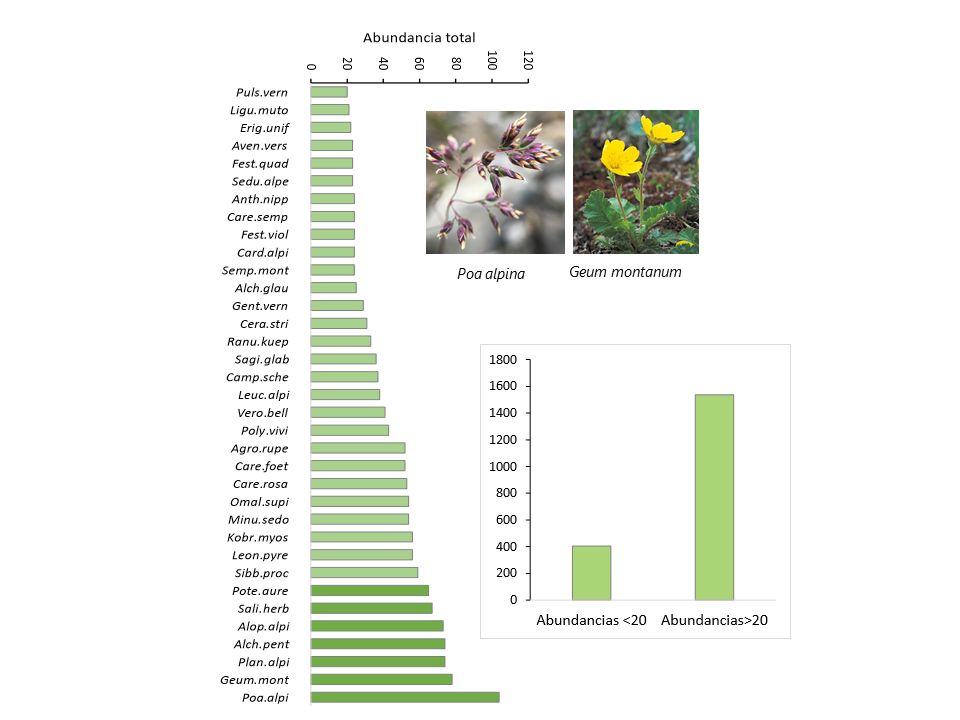
\includegraphics[width=5.65625in,height=\textheight]{figura_1_comp_especies.png}

}

\caption{\label{fig-abudancia}Abundancia total de especies encontradas.
En el gráfico inferior derecho se observa el recuento de especies que
presentaron abundancia superior o inferiores a 20 individuos. En el
gráfico izquierdo se presenta la abundancia de especies más dominantes.}

\end{figure}

En la Figure~\ref{fig-abudancia} se observa que las especies \emph{Poa
alpina} y \emph{Geum montanum} registran la mayor abundancia encontrada
(104 y 78 individuos respectivamente).

\includegraphics{images/tabla1.png}

\hypertarget{graficos-de-elipse}{%
\section{Graficos de elipse}\label{graficos-de-elipse}}

\includegraphics{images/elipse con correlación.png}

\includegraphics[width=5.625in,height=\textheight]{images/Imagen de WhatsApp 2024-03-14 a las 16.11.02_fe4b57b5.jpg}

Cajas y bigote

\begin{figure}

{\centering \includegraphics{images/Imagen de WhatsApp 2024-03-14 a las 16.11.49_b4775eec.jpg}

}

\caption{figura blogbox relacionando la perturbacion con la abundancia
usando como factor ZoogD}

\end{figure}

\hypertarget{referencias}{%
\section*{Referencias}\label{referencias}}
\addcontentsline{toc}{section}{Referencias}

\hypertarget{refs}{}
\begin{CSLReferences}{1}{0}
\leavevmode\vadjust pre{\hypertarget{ref-billings}{}}%
Billings, W. D. 1974. {``Adaptations and Origins of Alpine Plants*.''}
\emph{Arctic and Alpine Research} 6 (2): 129--42.
\url{https://doi.org/10.1080/00040851.1974.12003769}.

\leavevmode\vadjust pre{\hypertarget{ref-Choler2005-fq}{}}%
Choler, Philippe. 2005. {``Consistent Shifts in Alpine Plant Traits
Along a Mesotopographical Gradient.''} \emph{Arct. Antarct. Alp. Res.}
37 (4): 444--53.

\leavevmode\vadjust pre{\hypertarget{ref-dray2014}{}}%
Dray, Stéphane, Philippe Choler, Sylvain Dolédec, Pedro R. Peres-Neto,
Wilfried Thuiller, Sandrine Pavoine, and Cajo J. F. ter Braak. 2014.
{``Combining the Fourth{-}Corner and the RLQ Methods for Assessing Trait
Responses to Environmental Variation.''} \emph{Ecology} 95 (1): 14--21.
\url{https://doi.org/10.1890/13-0196.1}.

\end{CSLReferences}



\end{document}
